% Simple level diagram, resized and in a figure environment.
% Mark S. Everitt, 2009

\documentclass[10pt]{article}

% I only need the arrows for this one.
\usepackage{tikz}
\usetikzlibrary{arrows}
\usepackage{microtype}
%\usepackage{charter}
%\usepackage{palatino}
%\usepackage{newcent}
% \usepackage{bookman}
\usepackage{mathpazo}

% Nice captions.
\usepackage[hang,small,bf]{caption}
\setlength{\captionmargin}{25pt}

% New commands to keep things tidy.
\newcommand{\ket}[1]{$\left|#1\right\rangle$}
\newcommand{\Om}[1]{\small $\omega_{#1}$}
\newcommand{\De}[1]{$\Delta_{#1}$}
\newcommand{\Ga}[1]{$\Gamma_{#1}$}



\begin{document}

\section{Glossary}

For the purpose of this tutorial the following definitions will apply.

\begin{itemize}
    \item branch: a linked list of git commits where each commit is a node and has a parent and a child nodes.
    \item source: when applied to a branch refers to the name of another branch where the current one was grown from.
    \item remote: a repository where the local pull and push commands have effect on
    \item commit: a version of a file that can be computed as a delta or binary difference against a previous existing one.
    \item rebase: a git action and a concept whereby a series of commits from one branch are inserted into the same or another branch
    \item fast-forward: when a series of commits from a branch can be inserted, without any changes, at the tip of another branch because there are no conflicting commits.
    \item conflicting commit: when two or more commits affect the same parts of a file in ways that overlap each other.  
    \item merge: copying commits from one branch onto another starting at a specific commit
    \item local tree: the repository residing on the file system of the machine you are working in, as opposed to those that reside on a different machine or URL.
\end{itemize}

\section{Feature branch workflow}

The life cycle of a feature branch is to be created from its tree, receive new commits, be merged back into its tree and finally be deleted.
The quality of the history reflected by the tree will depend on how easy it is to interpret the tree.
In general the more linear the easier to understand as a timeline where file changes have happened at distinct points in time by specific contributors.

The workflow can be visualized through Figure~\ref{fig:feature-happy-path}. 
During the simultaneous growth of the branch and the main tree there is potential for conflicts if the contributions made at the same location in the same file are different, technically the branch and the main tree have diverged.

\begin{figure}
    \centering
    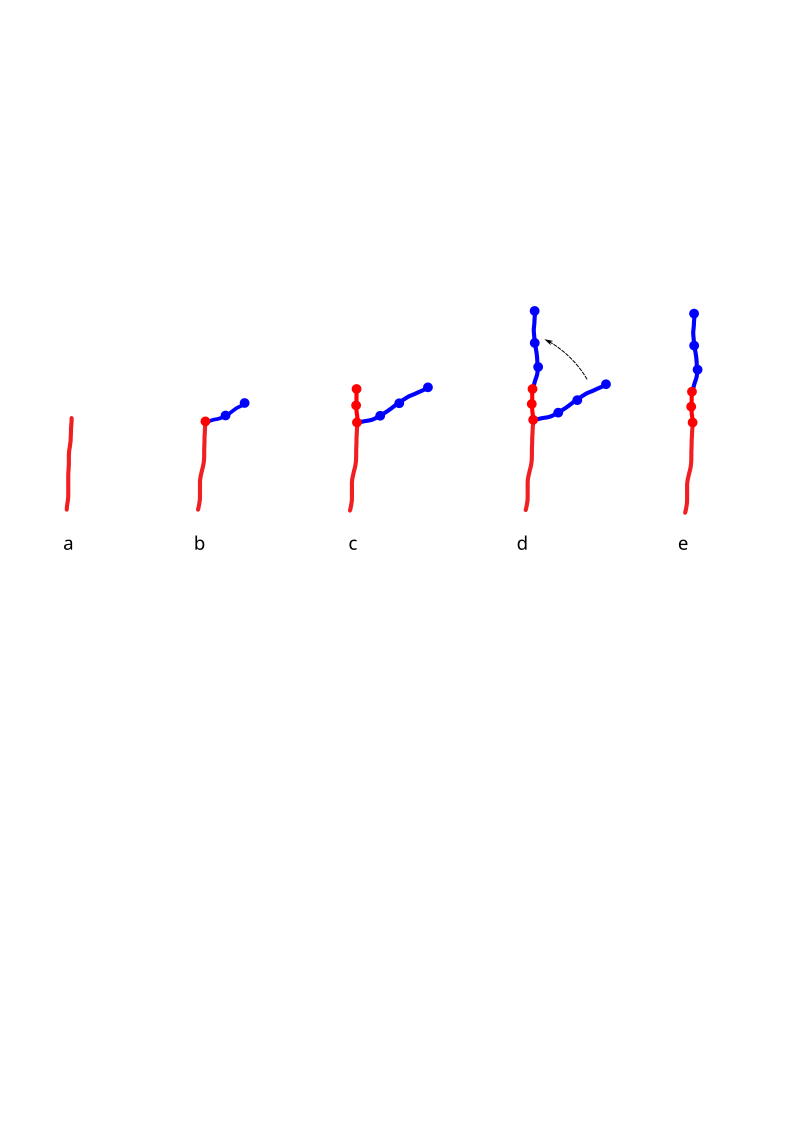
\includegraphics[width=\textwidth]{images/featurebranch_happy_path.png}
    \caption{Graphical representation of the history of a working tree when a feature branch is created. (a) The tree grows linearly, (b) the branch starts to grow, (c) both the branch and the main stem of the tree grow, (d) a copy of the branch is merged into the main stem, (e) the branch is removed.}
    \label{fig:feature-happy-path}
\end{figure}

In order to achieve this goal let's have a look at the best practice while using feature branches.
The workflow calls for two main git actions:

\begin{itemize}
    \item rebasing the source tree onto the feature branch as often as new commits appear on the source tree to address diverging histories.
    \item merging the feature branch into the source tree when the work is completed.
\end{itemize}

The first item, re-basing the source into the feature addresses potential conflicts created by the diverging timelines.

\section{Keeping the source branch up to date}

The ultimate goal of working with branches is to isolate change while work continues on the feature branch and on the origin branch.
When the origin branch in the local repository tracks a branch in an upstream remote, changes in the remote branch have to be pulled and re-based over the local branch.
By doing this, the final merge into the remote will look linear because the local changes will be brought a a simple  fast  forward merge without conflicts.

In this scenario the local repository has a branch called \textit{dev} that tracks a branch called the same name in the remote repository in a branch called \textit{origin}/\textit{dev}.
There is also a feature branch called \textit{feature} tracking \textit{origin}/\textit{feature}.

When there are new commits in \textit{origin}/\textit{dev} they should be brought into the local \textit{dev} branch via the following operation at the command line:

\begin{verbatim}
    (dev)$ git pull --rebase origin dev 
\end{verbatim}


Int he above snippet the \verb|(dev) $| piece indicates the current local branch name in parenthesis and the dollar symbol ios the command line prompt.


% A feature branch \textit{feature} created from a \textit{dev} branch has to be re-based periodically with the purpose of minimizing and simplifying the conflicts later on if they occur while merging it into \textit{dev}.
% The result will be a linear tree that is simple to read.


% Place the TikZ picture in a figure environment.
% \begin{figure}
% \centerline{
%   % Resize it to 5cm wide.
%   \resizebox{10cm}{!}{
%     \begin{tikzpicture}[
%       scale=0.5,
%       level/.style={thick},
%       virtual/.style={thick,densely dashed},
%       trans/.style={thick,<->,shorten >=2pt,shorten <=2pt,>=stealth},
%       classical/.style={thin,double,<->,shorten >=4pt,shorten <=4pt,>=stealth}
%     ]
%     % Draw the energy levels.
%     \draw[level] (0cm,11em) -- (7cm,11em) node[right] {Main};
%     \draw[level] (0cm,0em) -- (3cm,0em) node[right] {Dev};
%     % \draw[level] (2cm,11em) -- (4cm,11em) node[midway,above] {\ket{b}};
%     \draw[level] (0cm,-11em) -- (4cm,-11em) node[right] {Acc};
%     % Draw the virtual levels.
%     % \d1raw[virtual] (2cm,8em) -- (4cm,8em) node[midway,above] {\De{1}};
%     % \draw[virtual] (4cm,-8em) -- (6cm,-8em) node[midway,below] {\De{2}};
%     % \draw[virtual] (2cm,-5em) -- (0cm,-5em) node[midway,above] {\De{3}};
%     % % Draw the transitions.
%     % \draw[trans] (1cm,-2em) -- (2.5cm,8em) node[midway,left] {\Om{1}};
%     % \draw[trans] (3.5cm,8em) -- (5cm,-8em) node[midway,right] {\Om{2}};
%     % \draw[classical] (4.5cm,-8em) -- (1.5cm,-5em) node[midway,below] {\Ga{}};
%     \end{tikzpicture}
%   }
% }
% \caption{A level diagram with some transitions drawn in TikZ, resized,
%                 and placed in a figure environment.}
% \end{figure}

\end{document} 
